\chapter{Long Strings and the Black-Hole Correspondence}

\lectureoverview{A black hole has an entropy, so it must possess microscopic degrees of freedom. We shall build the simplest string-theoretic account of those degrees of freedom: first count the states of a long excited string, then vary the string coupling until the string and black-hole descriptions meet. The final equality is deliberately left as the problem to be completed in the next lecture.}

\section{Entropy Demands Microscopic Carriers}

To say that a system has a large entropy is to say that it can hide a large amount of microscopic information. A bathtub of hot water may have an entropy of order \(10^{30}\). That statement already tells us that there are enormously many microscopic degrees of freedom, whether or not we choose to inspect them molecule by molecule. Thermodynamics can determine the entropy by measuring energy and temperature, but it does not identify the objects that carry it.

Fluid dynamics makes the distinction familiar. It describes density, velocity, pressure, and macroscopic flow without referring to atoms. Add thermodynamics and one discovers that a fluid has entropy. The entropy announces a microscopic structure that the coarse-grained equations do not display; it invites a new question rather than answering it.

Black holes present the same challenge in a sharper form. Bekenstein's proposal, completed by Hawking's calculation, assigns entropy proportional to horizon area. General relativity determines the geometry and its thermodynamics, but it gives no inventory of the microscopic states. What are the small, numerous objects whose configurations account for the area law? In string theory there is a concrete candidate. The argument developed here is intentionally qualitative: it gets the parametric dependence right while suppressing numerical constants and the formal machinery of a full state count.

\section{Three Scales and One Notational Hazard}

Gravity supplies a distinguished length, the Planck length,
\begin{equation}
\ell_p=\sqrt{\frac{G_N\hbar}{c^3}}.
\label{eq:l06-planck-si}
\end{equation}

\begin{classroomqa}
\audiencequestion{Which combination of \(G_N\), \(\hbar\), and \(c\) gives the Planck length?\lecturetimestamp{00:06:08}}
\lecturerresponse{It is \(\sqrt{G_N\hbar/c^3}\), about \(10^{-33}\) centimeters. We shall immediately set \(\hbar=c=1\), so the relation becomes much simpler.}
\end{classroomqa}

In natural units,
\begin{equation}
\hbar=c=1,
\qquad
G_N=\ell_p^2.
\label{eq:l06-planck-area}
\end{equation}
Thus Newton's constant has dimensions of area. This is why an area divided by \(G_N\) is dimensionless and can be an entropy.

String theory has a second length, \(\ell_s\). Heat a string, or put it in a highly excited state, and it wiggles on many scales. The characteristic shortest scale in this elementary picture is the string length. One may regard \(\ell_s\) as the size associated with one elementary unit of string oscillation.

The third quantity is the dimensionless string coupling \(g_s\). It controls splitting and joining: a string can pinch into two strings, or an excited string can emit a closed-string quantum.

\begin{classroomqa}
\audiencequestion{What is the physical meaning of the string coupling?\lecturetimestamp{00:09:20}}
\lecturerresponse{It controls the chance for a string interaction, such as splitting when a string crosses itself. More precisely, \(g_s\) is the interaction amplitude; a corresponding probability or rate begins at order \(g_s^2\).}
\end{classroomqa}

The emitted massless closed-string excitation can be a graviton. In that respect \(g_s\) plays a role analogous to electric charge: it is the factor attached to an interaction vertex.\editorialnote{The lecture alternates between calling \(g_s\) a probability and an amplitude. Perturbatively it is the amplitude-level coupling; probabilities and rates contain its square.}

\section{Why Gravity Knows About \texorpdfstring{\(g_s^2\)}{the Coupling Squared}}

Consider first the exchange picture for electromagnetism. One charged object emits a photon with a factor of \(e\), and a second absorbs it with another factor of \(e\). The exchange amplitude therefore contains \(e^2\). The picture is not a literal classical projectile story, but it correctly displays how the coupling enters.

\begin{figure}[htbp]
\centering

\includegraphics[width=0.72\textwidth]{lecture_06_figure_03.png}
\caption{The completed exchange sketches on the board: a coupling is attached at emission and again at absorption.}
\lectureframe{00:11:30.000}
\end{figure}

The string-theory version replaces the photon by a graviton and the electric charge by \(g_s\). One factor accompanies emission and another absorption, so the gravitational strength scales as \(g_s^2\).

At long distance the same interaction must reproduce Newton's force law,
\begin{equation}
F_{\mathrm{grav}}\sim G_N\frac{M_1M_2}{r^2}.
\end{equation}
The masses and inverse-square dependence describe the sources and propagation; the point needed here is the coupling multiplying them.

\begin{figure}[htbp]
\centering
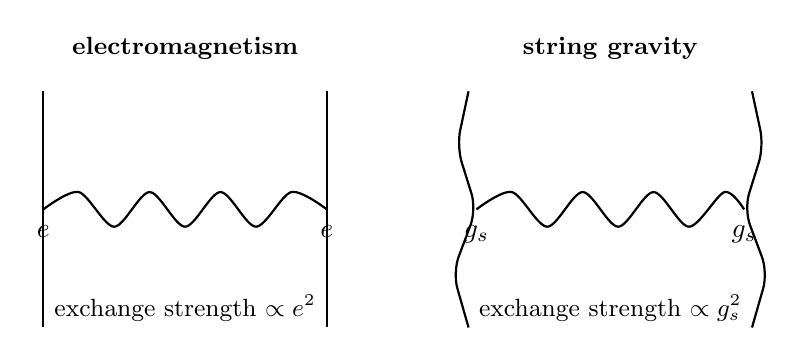
\begin{tikzpicture}[x=1cm,y=1cm]
  \node[font=\small\bfseries] at (1.8,3.55) {electromagnetism};
  \draw[line width=0.8pt] (0,0) -- (0,3);
  \draw[line width=0.8pt] (3.6,0) -- (3.6,3);
  \draw[line width=0.8pt] plot[smooth] coordinates {(0,1.5) (0.45,1.72) (0.9,1.28) (1.35,1.72) (1.8,1.28) (2.25,1.72) (2.7,1.28) (3.15,1.72) (3.6,1.5)};
  \node[below] at (0,1.42) {\(e\)};
  \node[below] at (3.6,1.42) {\(e\)};
  \node[font=\small] at (1.8,0.25) {exchange strength \(\propto e^2\)};
  \node[font=\small\bfseries] at (7.2,3.55) {string gravity};
  \draw[line width=0.8pt,rounded corners=6pt] (5.4,0) -- (5.2,0.7) -- (5.5,1.5) -- (5.25,2.3) -- (5.4,3);
  \draw[line width=0.8pt,rounded corners=6pt] (9,0) -- (9.2,0.7) -- (8.9,1.5) -- (9.15,2.3) -- (9,3);
  \draw[line width=0.8pt] plot[smooth] coordinates {(5.5,1.5) (5.95,1.72) (6.4,1.28) (6.85,1.72) (7.3,1.28) (7.75,1.72) (8.2,1.28) (8.65,1.72) (8.9,1.5)};
  \node[below] at (5.5,1.42) {\(g_s\)};
  \node[below] at (8.9,1.42) {\(g_s\)};
  \node[font=\small] at (7.2,0.25) {exchange strength \(\propto g_s^2\)};
\end{tikzpicture}
\caption{The coupling-counting analogy. Each end of the exchanged quantum contributes one interaction factor.}
\end{figure}

This observation almost determines Newton's constant. The coupling \(g_s\) is dimensionless, while in four dimensions \(G_N\) has dimensions of length squared. The available microscopic length is \(\ell_s\), hence
\begin{equation}
G_N\sim g_s^2\ell_s^2.
\label{eq:l06-newton-string}
\end{equation}
Combining this with Equation~\eqref{eq:l06-planck-area} gives
\begin{equation}
\ell_p\sim g_s\ell_s.
\label{eq:l06-planck-string}
\end{equation}

\begin{figure}[htbp]
\centering

\includegraphics[width=0.72\textwidth]{lecture_06_figure_04.png}
\caption{The basic relations retained on the board: \(\ell_p^2=G_N\) and \(\ell_p\sim g_s\ell_s\).}
\lectureframe{00:15:45.000}
\end{figure}

Equation~\eqref{eq:l06-newton-string} is the simplified relation used throughout this lecture.\editorialnote{In a compactified string theory the effective four-dimensional Newton constant also depends on the compactification volume and order-one conventions. The lecture suppresses those data to isolate the correspondence scaling.}

\begin{classroomqa}
\audiencequestion{Is \(g_s\) greater or less than one, and which length is larger?\lecturetimestamp{00:16:00}}
\lecturerresponse{We work at weak coupling, \(g_s<1\). Then \(\ell_p\sim g_s\ell_s\) implies that the string length is larger than the Planck length. Strong coupling requires a different description and is not needed here.}
\end{classroomqa}

\section{The Black-Hole Count}

Suppressing Boltzmann's constant and numerical factors, the Bekenstein--Hawking entropy is
\begin{equation}
S_{\mathrm{BH}}=\frac{A}{4G_N}sim\frac{A}{G_N}sim\frac{A}{\ell_p^2}.
\label{eq:l06-bh-area}
\end{equation}
The factor \(1/4\) is exact in the semiclassical formula, but it will play no role in this scaling argument.

\begin{classroomqa}
\audiencequestion{Does the subscript ``BH'' mean black hole or Bekenstein--Hawking?\lecturetimestamp{00:16:51}}
\lecturerresponse{For our purposes it can remind us of both. The important statement is that the entropy is the horizon area measured in Planck areas.}
\end{classroomqa}

For a four-dimensional Schwarzschild black hole,
\begin{equation}
R_s=2G_NM,
\qquad
A=4\pi R_s^2.
\end{equation}
Dropping \(2\) and \(4\pi\) as the lecture does,
\begin{align}
S_{\mathrm{BH}}
&\sim \frac{R_s^2}{G_N}
\sim \frac{(G_NM)^2}{G_N} \\
&\sim M^2G_N
\sim M^2\ell_p^2.
\label{eq:l06-bh-mass}
\end{align}
This is the form we shall compare with a string count.

\section{A Long String as a Random Walk}

Begin with a small string and pump energy into it. A generic highly excited string does not remain a tidy loop. It becomes a long, tangled object, like fishing line after a badly snarled reel. The tangle has entropy because a huge number of configurations look macroscopically alike.

To count them, replace space by a lattice whose links have length \(\ell_s\). Sites are the vertices, links are the lines, and the elementary squares are plaquettes. A string is represented by a connected sequence of links. This model is deliberately crude, but its exponential state count captures the desired scaling.

\begin{figure}[htbp]
\centering

\includegraphics[width=0.72\textwidth]{lecture_06_figure_05.png}
\caption{The two-dimensional lattice model. The blue segment marks one step of the string; the four possible continuations are counted at each site.}
\lectureframe{00:23:50.000}
\end{figure}

\begin{classroomqa}
\audiencequestion{How many choices are there at each step of the toy walk?\lecturetimestamp{00:22:43}}
\lecturerresponse{Four on the square lattice, since immediate backtracking is allowed. In three dimensions there would be six. Another lattice changes the ordinary number but not the fact that the number of walks grows exponentially with the number of links.}
\end{classroomqa}

If the string has \(n\) links, the two-dimensional toy count is
\begin{equation}
\Omega_n\sim4^n.
\label{eq:l06-walk-count}
\end{equation}
There is one exceptional straight walk, but it is only one state among \(4^n\). A typical walk folds repeatedly and occupies a tangled ball. For large \(n\), almost every randomly generated configuration looks qualitatively like every other one.

The entropy is the logarithm of the number of macroscopically indistinguishable configurations:
\begin{equation}
S_{\mathrm{st}}=\log\Omega_n\sim n\log4\sim n.
\label{eq:l06-string-entropy-n}
\end{equation}

\begin{classroomqa}
\audiencequestion{Why does the entropy become proportional to \(n\) rather than to \(4^n\)?\lecturetimestamp{00:25:39}}
\lecturerresponse{Entropy is the logarithm of the number of states. Thus \(\log(4^n)=n\log4\), and the factor \(\log4\) is an order-one constant that we shall suppress.}
\end{classroomqa}

If \(L\) is the contour length obtained by following the string from one end to the other, then
\begin{equation}
n=\frac{L}{\ell_s},
\qquad
S_{\mathrm{st}}\sim\frac{L}{\ell_s}.
\label{eq:l06-string-entropy-length}
\end{equation}
Here \(L\) is not the diameter of the tangled ball. It is the much longer distance measured along the string.

We next trade contour length for mass. With \(c=\hbar=1\), mass has dimensions of inverse length. One string-sized link therefore carries mass of order
\begin{equation}
m_{\mathrm{link}}\sim\frac{1}{\ell_s}.
\label{eq:l06-link-mass}
\end{equation}

\begin{classroomqa}
\audiencequestion{Why must the mass of one link scale as \(1/\ell_s\)?\lecturetimestamp{00:29:20}}
\lecturerresponse{In these units mass is an inverse length, and \(\ell_s\) is the only available length. Equivalently, a string tension of order \(1/\ell_s^2\) multiplied by a link length \(\ell_s\) gives the same result.}
\end{classroomqa}

The full string then has
\begin{equation}
M\sim n m_{\mathrm{link}}
\sim\frac{n}{\ell_s}
\sim\frac{L}{\ell_s^2},
\qquad
L\sim M\ell_s^2.
\label{eq:l06-string-mass}
\end{equation}
Substitution into Equation~\eqref{eq:l06-string-entropy-length} yields
\begin{equation}
S_{\mathrm{st}}\sim M\ell_s.
\label{eq:l06-string-entropy-mass}
\end{equation}
The lattice walk ignores world-sheet constraints and numerical coefficients, but the exponential growth of the highly excited string spectrum gives this same leading scaling.\editorialnote{The random-walk construction is a mnemonic for the high-level density of string states, not a literal discretization of a fundamental string.}

\section{The Mismatch That Starts the Argument}

The two answers are now
\begin{equation}
S_{\mathrm{BH}}\sim M^2\ell_p^2,
\qquad
S_{\mathrm{st}}\sim M\ell_s.
\label{eq:l06-two-entropies}
\end{equation}
They resemble one another, but they are not equal at fixed mass and arbitrary coupling. The black-hole expression is quadratic in \(M\); the string expression is linear. A hot string cannot simply be declared to be a black hole without explaining how the two regimes meet.

\begin{figure}[htbp]
\centering

\includegraphics[width=0.78\textwidth]{lecture_06_figure_06.png}
\caption{The unobstructed board comparison: black-hole entropy above, long-string entropy below, with the Planck--string relations retained at left.}
\lectureframe{00:33:20.000}
\end{figure}

This is where the class paused. The suspense is useful: the mismatch is not a failure of the idea but the clue that one must compare the same state while changing the strength of gravity.

\section{Turning the Coupling Dial}

Hold \(\ell_s\) fixed and imagine that \(g_s\) can be varied. At \(g_s=0\), strings neither split nor join and gravity vanishes because \(G_N\sim g_s^2\ell_s^2\). A sufficiently energetic state is then a long, weakly interacting string.

Increase \(g_s\) slowly. String interactions become possible and, more importantly for the present argument, gravity strengthens.

\begin{classroomqa}
\audiencequestion{As \(g_s\) increases, is the first effect simply that the string splits into shorter strings?\lecturetimestamp{00:36:29}}
\lecturerresponse{Splitting and joining become possible, but hold \(\ell_s\) fixed and follow the high-entropy state. The central effect is that \(G_N\) grows, so the long string's self-gravity pulls the tangled ball inward.}
\end{classroomqa}

The object contracts and becomes denser. Its gravitational potential energy is negative, so contraction lowers its total energy and therefore its mass.

\begin{classroomqa}
\audiencequestion{Does the energy increase or decrease as self-gravity pulls the string together?\lecturetimestamp{00:37:48}}
\lecturerresponse{It decreases. The binding energy becomes more negative. The mass along the path need not remain fixed even though we continue to follow the same state.}
\end{classroomqa}

Eventually the object's size is comparable to its Schwarzschild radius. Beyond that point the black-hole description is the natural one. A larger initial excitation reaches this condition at a smaller coupling because a more massive object requires less gravitational strength to form a horizon.

\begin{figure}[htbp]
\centering
\resizebox{0.95\linewidth}{!}{%
\begin{tikzpicture}[x=1cm,y=1cm,>=Latex]
  \draw[->,line width=0.9pt] (0,0) -- (11,0) node[right] {increasing \(g_s\)};
  \node[draw,rounded corners,align=center,minimum width=2.6cm,minimum height=1.15cm] at (1.8,1.5) {long excited string\\weak self-gravity};
  \node[draw,rounded corners,align=center,minimum width=2.6cm,minimum height=1.15cm] at (5.5,1.5) {correspondence point\\\(R_s\sim\ell_s\)};
  \node[draw,circle,align=center,minimum size=1.8cm] at (9.3,1.5) {black\\hole};
  \draw[->,line width=0.8pt] (3.15,1.5) -- (4.1,1.5) node[midway,above,font=\small] {contracts};
  \draw[->,line width=0.8pt] (6.9,1.5) -- (8.25,1.5);
  \node[font=\small,align=center] at (5.5,-0.65) {same family of states followed slowly;\\binding energy and mass may change};
\end{tikzpicture}
}
\caption{The correspondence path at fixed \(\ell_s\). Reversing the arrow takes the black-hole state back to a long-string state.}
\end{figure}

\begin{classroomqa}
\audiencequestion{Should we imagine \(g_s\) between zero and one?\lecturetimestamp{00:40:18}}
\lecturerresponse{Yes. The argument remains in the weak-coupling regime. If \(g_s\) is very small, the state must be correspondingly massive before it becomes a black hole. We do not need to enter the poorly controlled \(g_s>1\) regime.}
\end{classroomqa}

The slow change is reversible in the thought experiment.

\begin{classroomqa}
\audiencequestion{If we turn the coupling back down until gravity can no longer hold the black hole together, what does it become?\lecturetimestamp{00:41:37}}
\lecturerresponse{A long string. At vanishing gravity everything in this construction must be described in string states. Turning the dial one way maps string to black hole; turning it back maps black hole to string.}
\end{classroomqa}

At fixed total energy and within a fixed volume, the dominant high-entropy configuration is essentially one long string rather than an enormous number of short strings. That statement is not derived here. It is a result of the statistical mechanics of strings near the Hagedorn regime and will be revisited.

\section{What the Outside Observer Sees}

Where is the string when the object is described as a black hole? In the outside description it does not abruptly disappear. Schwarzschild time sends the apparent crossing to arbitrarily late time, so the stringy degrees of freedom are represented as accumulating on or near the horizon.

\begin{figure}[htbp]
\centering

\includegraphics[width=0.72\textwidth]{lecture_06_figure_07.png}
\caption{The board comparison between a macroscopic horizon, where string-scale structure is a thin fuzz, and a smaller horizon whose radius approaches the loop scale.}
\lectureframe{00:45:30.000}
\end{figure}

For \(R_s\gg\ell_s\), the black hole is macroscopic and the string-scale structure is only a thin layer relative to the horizon radius. As the radius decreases toward \(\ell_s\), the distinction between a smooth black hole and an extended string loses meaning. This is an outside, stretched-horizon description; it should not be confused with a coordinate-independent claim that infalling matter never crosses a regular horizon.\editorialnote{The lecture uses the exterior description familiar from black-hole complementarity. The phrase ``on the horizon'' denotes degrees of freedom resolved by the outside description, not a separate derivation of their covariant location.}

The crossover occurs when
\begin{equation}
R_s\sim\ell_s.
\label{eq:l06-correspondence-radius}
\end{equation}
Below the string scale, the Schwarzschild geometry cannot resolve the structure that is supposed to support it. The loops fluctuate away from the would-be horizon, and the state is better called a string.

\section{The Correspondence Point}

Use \(R_s\sim G_NM\) in Equation~\eqref{eq:l06-correspondence-radius}:
\begin{equation}
G_NM\sim\ell_s.
\end{equation}
Then substitute \(G_N\sim g_s^2\ell_s^2\):
\begin{equation}
M g_s^2\ell_s^2\sim\ell_s,
\qquad
M g_s^2\ell_s\sim1.
\label{eq:l06-correspondence-condition}
\end{equation}

\begin{figure}[htbp]
\centering

\includegraphics[width=0.72\textwidth]{lecture_06_figure_08.png}
\caption{The completed transition algebra on the board: \(R_s\sim\ell_s\) leads to the boxed dimensionless condition \(Mg_s^2\ell_s\sim1\).}
\lectureframe{00:49:50.000}
\end{figure}

An audience member noticed what this condition is preparing. At the correspondence point,
\begin{align}
S_{\mathrm{BH}}
&\sim M^2\ell_p^2
\sim M^2g_s^2\ell_s^2 \\
&=(M\ell_s)(Mg_s^2\ell_s)
\sim M\ell_s
\sim S_{\mathrm{st}}.
\label{eq:l06-entropy-preview}
\end{align}

\begin{classroomqa}
\audiencequestion{Do the equations already imply that the black-hole and string entropies become equal?\lecturetimestamp{00:50:18}}
\lecturerresponse{Yes. That is exactly where the calculation is going. The ingredients have been placed on the board, but the lecture postpones their full assembly so that the logic of the correspondence can be reviewed carefully.}
\end{classroomqa}

Equation~\eqref{eq:l06-entropy-preview} is the one-line algebraic preview implicit in the exchange. It establishes the scaling, not the exact coefficient \(1/4\). Exact microscopic matches require more controlled black holes and more detailed string constructions.\editorialnote{The lecture stops before presenting Equation~\eqref{eq:l06-entropy-preview} as its completed derivation. It is written out here because the audience explicitly identifies the equality and every required relation has already appeared.}

\section{Why the Entropy Can Be Carried Across}

One logical ingredient remains. Suppose a control parameter, such as a magnetic field or \(g_s\), is varied sufficiently slowly while the system is isolated and the evolution is reversible. Energies, sizes, and binding may change, but the entropy is preserved:
\begin{equation}
\Delta S=0.
\label{eq:l06-adiabatic-entropy}
\end{equation}
The lecture connects this to conservation of information. Entropy measures information hidden by a coarse-grained description; a slow reversible change of the Hamiltonian rearranges the states without deleting that information.

\begin{classroomqa}
\audiencequestion{Does constant entropy require that the path avoid a phase transition?\lecturetimestamp{00:54:01}}
\lecturerresponse{Yes, one must be able to follow the state continuously. A finite system has no strictly nonanalytic thermodynamic phase transition of the infinite-volume kind, and if the change is slow enough the correspondence can be treated as a smooth crossover.}
\end{classroomqa}

Adiabatic is being used here in the stronger quasistatic, reversible sense. An adiabatic but irreversible process can produce entropy; slowness and the ability to track the state are essential.\editorialnote{The thermodynamic statement \(\Delta S=0\) requires a reversible adiabatic path. Quantum mechanically, the corresponding idea is to follow the same set of states as a parameter changes without uncontrolled level transitions.}

\begin{classroomqa}
\audiencequestion{Why should one long string have more entropy than several shorter strings carrying the same total mass?\lecturetimestamp{00:54:44}}
\lecturerresponse{It is counterintuitive, but the explicit high-energy state count favors a long-string component in a fixed volume. The proof is deferred; for the present argument we need only that the black hole maps to the maximum-entropy string sector rather than to a dilute gas of very many short strings.}
\end{classroomqa}

The operational strategy is therefore:
\begin{enumerate}
\item Begin with a black hole of mass \(M_0\) at coupling \(g_{s,0}\).
\item Lower \(g_s\) slowly while following the same high-entropy family of states.
\item Stop at \(R_s\sim\ell_s\), where the black-hole description becomes a long-string description.
\item Count the string states using \(S_{\mathrm{st}}\sim M\ell_s\).
\item Carry that entropy back along the reversible path to the original black hole.
\end{enumerate}

\begin{figure}[htbp]
\centering

\includegraphics[width=0.72\textwidth]{lecture_06_figure_09.png}
\caption{The principle retained on the board while the strategy is stated: an adiabatic change of \(g_s\) does not change \(S\).}
\lectureframe{00:56:40.000}
\end{figure}

String theory has produced much sharper entropy counts for charged, rotating, supersymmetric, near-extremal, and higher-dimensional black holes. The neutral Schwarzschild discussion here is the rough correspondence argument: it identifies the parametric density of states and the physical crossover, not an exact protected degeneracy.\editorialnote{Exact agreement is strongest for special black holes whose state counts are protected as the coupling changes. The present lecture intentionally gives the simplest order-of-magnitude version.}

\begin{classroomqa}
\audiencequestion{Could the state become two strings rather than exactly one when gravity is turned off?\lecturetimestamp{00:58:25}}
\lecturerresponse{There is a finite probability for a small number of long strings, and using two rather than one does not change the leading entropy scaling. What would change the argument is fragmentation into a huge gas of short strings; the high-energy statistical count does not favor that outcome.}
\end{classroomqa}

The black hole is the greatest entropy that can be packed into a region, and the long string is the corresponding high-entropy state when gravity is removed. Those two descriptions are now connected, but not yet developed into a precision calculation. The next step is to repeat the algebra carefully and ask how far the correspondence can be trusted.
